\section{Test-bed Environment and Experiments}
\label{sec:evaluation}

\subsection{Frontend testing}
When developing the frontend of our application, multiple testing strategies were performed to make sure that the 
application's functionalities were behaving as expected. One of the advantages of using Angular, is that it provides 
the option to do real-time compilation of the application. This feature made it possible to view the results immediately 
after code changes. This shortened the time spent on troubleshooting errors. The inspect tool in the browser were 
also a great tool that quickly let us inspect the applications. The console feature were handy when inspecting the 
HTML and CSS, and the Network analysis tool gave us a great insight into how the frontend and the backend 
communicated. Alerts were also created to notify the user whenever errors and issues occurred. 
of errors 

\subsection{JUnit testing}
The purpose of the JUnit tests is to verify our application's functionality. Using a mocking framework, they imitate particular application components, enabling targeted testing of individual functionalities without requiring the entire system. Important components analyzed are:

\begin{itemize}
    \item The ability of the application to successfully retrieve all items from a list, such as all users or polls.
    \item Capability to find a specific item by its unique identifier.
    \item Correct behavior of the application when an item cannot be found.
    \item The functionality to add, update, or remove items effectively.
\end{itemize}

Expected results, such as the quantity of objects recovered or the reaction in the event that an item is missing, are confirmed in each test. These tests are essential to ensure the application functions as expected.

\subsection{Postman testing}
Postman is a popular tool for testing REST APIs. It allows us to query the API endpoints of our application and receive back responses. The most important features tested using Postman include:

\begin{itemize}
    \item {Sending Different Types of Requests}: Postman test various request types like GET, POST, PUT, and DELETE. These are essential for operations in our application such as getting, creating, updating, or deleting data.
    \item {Verifying Responses}: The tool can verify whether the API returned the correct data and response codes. For instance, confirming that a GET request fetches the right list of items, or a 404 status code is returned when an item is not found.
    \item {Parameter Testing}: Postman allows testing how the API handles different parameters, such as specific item searches or result filtering.
    \item {Error Handling}: By sending incorrect or incomplete requests, we can test the API's error handling and check if it returns appropriate error messages.
\end{itemize}

\begin{figure}[h]
  \centering
  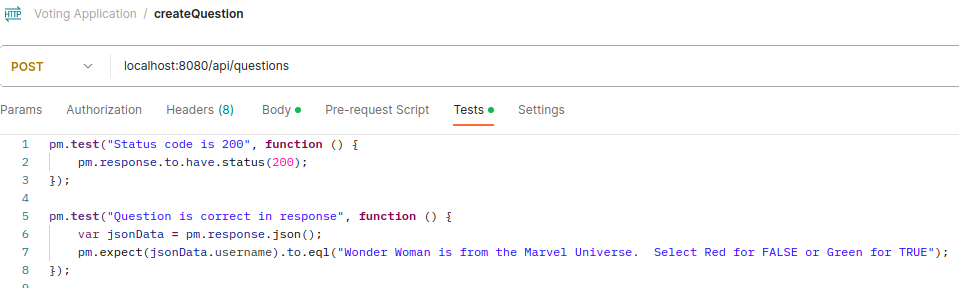
\includegraphics[scale=0.65]{figs/create_question_test.png}
  \caption{Sample Postman Test}
  \label{fig:appFlow}
\end{figure}

\noindent These tests make sure that our application's API is reliable, and performs as expected under different scenarios.

\subsection{IoT Device testing}

Testing of IoT device was testing using an informal and dynamic approach.  Instead of defining specific test cases, we relied on our domain knowledge, experience and creativity to find defects.  Using this type of testing allowed us to design, implment and test simultaneiously, enabling us to uncover design and development defects continiously in the software development loop. 